\chapter{观测设计、误差预算与可行性}
\label{chap:e15}

\begin{chapteropening}
到这里为止，我们已经把工具箱配齐了：第 \ref{chap:e11} 章告诉我们强度干涉的信噪比怎样随望远镜面积、光子率和积分时间标度；第 \ref{chap:e12} 章告诉我们一份数据里到底藏着多少可提取的信息（Fisher 信息与 Cramér--Rao 下界）；第 \ref{chap:e13} 章交代了探测器、时钟和事件表，第 \ref{chap:e14} 章交代了相关器怎样把事件表变成 \(g^{(2)}(\tau)\) 和 \(|V|^2(B)\)。现在要做的，是把这些零件\textbf{攒成一次真实的观测}。想象你面前是一张空白的观测申请表：你要观测哪颗星？用几台望远镜、多长基线、多宽的滤光片？曝多久？最后能把角直径测到百分之几？——这一章就是从头到尾把这张表填满的过程。核心是一张\textbf{账本}：光子率给出统计上限，相关对比度（contrast）给出目标信号，基线、带宽、时间分辨率和定标误差决定这个信号能不能从噪声里活下来。我们会把每一步都算成真实数字，最后走一遍从一颗真实亮星到一个可达精度的完整可行性计算。
\end{chapteropening}

\section{一次观测就是一张从参数到数据的账本}
\label{sec:e15-ledger}

每一次观测，追根究底都是为了估计几个物理数。恒星的角直径、双星的角间距、快速自转星的扁率和长轴方向、谱线发射区的半径、偏振角的旋转、两路信号的时延、二阶相关峰的高度——这些就是我们真正想要的\textbf{物理参数}（physical parameters），记作 \(\bm\theta_{\rm phys}\)。可仪器交给我们的，从来不是这些数，而是第 \ref{chap:e13} 章讲过的\textbf{事件表}（event list）：一行一个光子，带着到达时间、望远镜编号、波长和偏振标签。物理参数要从这些字段里\emph{反推}出来。

于是设计一次观测，第一件事不是问"我想看哪颗星"，而是问"我要的数，事件表里有没有支撑它的字段"。要做纳秒级时间相关，时间戳的精度就得压到纳秒；要给出所需基线，位置标签就得记准；要分波段或测偏振，波长和偏振标签就不能在记录时被抹掉。这里有一条容易被忽视却致命的原则：\textbf{信息一旦在记录环节被平均掉，后期再也补不回来}。如果你一开始只存一张长时间积分的图像，那么纳秒时间相关、偏振相关都已经随平均消失了；而如果你老老实实存下整张事件表，后面就能把它任意投影成光变曲线、\(g^{(2)}(\tau)\)、\(|V|^2(B)\)、偏振角，或者多波长的 \(u,v\) 数据。事件表是"原汤"，图像只是"熬干后的一勺"。

从参数到数据的整条链，可以写成一个似然：

\begin{equation}
  \mathcal L(\bm\theta_{\rm phys})
  =
  P\!\left(\,d \;\middle|\;
  q_{\rm inst}(\bm\theta_{\rm phys}),\;
  \bm c_{\rm cal},\;
  \bm b_{\rm sky}
  \right).
  \label{eq:e15-likelihood}
\end{equation}
\begin{formulaexplain}
\(\bm\theta_{\rm phys}\)：要估计的物理参数（如角直径 \(\theta\)）。\(d\)：观测到的数据或其统计量。\(q_{\rm inst}\)：仪器真正测到的量（如 \(|V|^2\)）。\(\bm c_{\rm cal}\)：定标参数。\(\bm b_{\rm sky}\)：天空背景。这条式子在说：物理参数先被仪器"翻译"成可测量，再和定标、背景一起决定数据出现的概率。
\end{formulaexplain}

逐个符号落地。\(\mathcal L\) 是似然（likelihood），无量纲，衡量"若真参数是 \(\bm\theta_{\rm phys}\)，看到这份数据 \(d\) 的概率有多大"。\(q_{\rm inst}\) 是仪器可测量：可以是平方可见度 \(|V|^2\)（无量纲）、二阶相关的超出量 \(g^{(2)}-1\)（无量纲）、偏振 Stokes 分量，或到达时间残差（秒）。\(\bm c_{\rm cal}\) 是定标参数——时间零点、滤光片通带、探测器效率、增益状态——它们不是我们想要的物理量，却会污染数据，必须一并估计或事先测定。\(\bm b_{\rm sky}\) 是天光、月光、暗计数和宿主星系背景。写观测申请时，与其空泛地说"我们会观测这颗星"，真正有用的是把这条链算穿：这颗星的星等 \(m_B\) 是多少、角直径 \(\theta\) 估计多大、可见窗口有多长、模型先验会给出哪几个 \(|V|^2\) 数据点、最终能把 \(\theta\) 的误差压到百分之几。本章余下几节，就是逐段把这条链填成真实数字。

\section{光子预算：从星等到有效光子数}
\label{sec:e15-photon-budget}

一切从光子率开始。一颗星再有意思，如果每秒只给你几个光子，任何相关信号都会淹没在噪声里。所以可行性计算的第一步，永远是把\textbf{星等翻译成每秒光子数}。这条翻译分四步：星等 \(\to\) 谱流量密度 \(\to\) 单位面积光子通量 \(\to\) 乘上面积与效率得到有效光子率。我们一步一步来。

\paragraph{第一步：星等到谱流量密度}

天文学用星等（magnitude）描述亮度，星等每小 5 等，亮度大 100 倍——这是一把对数尺子。AB 星等的好处是它直接对应谱流量密度：

\begin{equation}
  F_\nu = 3631\,{\rm Jy}\times 10^{-0.4\,m_{\rm AB}}.
  \label{eq:e15-ab-flux}
\end{equation}
\begin{formulaexplain}
\(m_{\rm AB}\)：AB 星等（无量纲）。\(F_\nu\)：单位频率的谱流量密度。\(1\,{\rm Jy}=10^{-23}\,{\rm erg\,s^{-1}\,cm^{-2}\,Hz^{-1}}\)。常数 \(3631\,{\rm Jy}\) 是 \(m_{\rm AB}=0\) 的定义流量。星等每增 5，\(F_\nu\) 降 100 倍。
\end{formulaexplain}

这里 \(F_\nu\) 是谱流量密度，量纲是"能量 / (时间·面积·频率)"，CGS 单位为 \({\rm erg\,s^{-1}\,cm^{-2}\,Hz^{-1}}\)；\(1\,{\rm Jy}\)（央斯基）\(=10^{-23}\) 这个单位。取一颗 \(m_{\rm AB}=5\) 的星，代入即得
\[
  F_\nu = 3631\,{\rm Jy}\times 10^{-0.4\times5}
        = 3631\times10^{-2}\,{\rm Jy}
        = 36.3\,{\rm Jy}
        = 3.63\times10^{-22}\,{\rm erg\,s^{-1}\,cm^{-2}\,Hz^{-1}} .
\]
这就是这颗星在每一赫兹频率上，每秒穿过每平方厘米的能量。数字很小——一平方厘米、一赫兹带宽，一秒钟才收到 \(10^{-22}\) 尔格，这提醒我们后面必须靠大面积和宽带宽把它攒起来。

\paragraph{第二步：能量流量到光子通量}

探测器数的不是能量，是光子个数。一个频率 \(\nu\) 的光子带能量 \(h\nu\)（\(h=6.63\times10^{-27}\,{\rm erg\,s}\) 是普朗克常数）。把能量流量除以单光子能量，就得到单位面积、单位时间、单位带宽的光子数。再乘上光学带宽 \(\Delta\nu\)，就得到整条通带每平方厘米每秒的光子数。带宽换算沿用第 \ref{chap:e02} 章的关系 \(\Delta\nu\simeq c\,\Delta\lambda/\lambda^2\)。取观测波长 \(\lambda=550\,{\rm nm}\)、通带 \(\Delta\lambda=10\,{\rm nm}\)：
\[
  \nu=\frac{c}{\lambda}=\frac{3\times10^{10}\,{\rm cm\,s^{-1}}}{550\times10^{-7}\,{\rm cm}}
     =5.45\times10^{14}\,{\rm Hz},
  \qquad
  h\nu = 6.63\times10^{-27}\times5.45\times10^{14}
       = 3.61\times10^{-12}\,{\rm erg},
\]
\[
  \Delta\nu = \frac{c\,\Delta\lambda}{\lambda^2}
            = \frac{3\times10^{10}\times10\times10^{-7}}{(550\times10^{-7})^2}
            = 9.9\times10^{12}\,{\rm Hz}\approx10^{13}\,{\rm Hz}.
\]
于是单位面积光子通量
\[
  \Phi = \frac{F_\nu\,\Delta\nu}{h\nu}
       = \frac{3.63\times10^{-22}\times 9.9\times10^{12}}{3.61\times10^{-12}}
       \approx 1.0\times10^{3}\ {\rm photons\,s^{-1}\,cm^{-2}} .
\]
一平方厘米、10 nm 通带，每秒约一千个光子——这是\emph{到达大气层顶}的、还没打折的原始通量。

\paragraph{第三步：乘面积与效率，得到有效光子率}

真正落进相关器的光子，还要乘两个因子：望远镜的\textbf{有效收集面积}\(A\)，和从大气到光子计数的\textbf{总效率}\(\eta\)。后者把大气透过率、镜面反射率、滤光片透过率、光纤耦合损失和探测器量子效率（quantum efficiency，见第 \ref{chap:e07} 章）全部并进一个数，典型值 \(\eta\sim0.2\)--\(0.3\)。合起来：

\begin{equation}
  R_\gamma
  = \eta\,A\,\frac{F_\nu\,\Delta\nu}{h\nu}
  = \eta\,A\,\Phi .
  \label{eq:e15-photon-rate}
\end{equation}
\begin{formulaexplain}
\(R_\gamma\)：有效光子率（每秒计数）。\(\eta\)：总效率（无量纲，含大气、镜面、滤光片、探测器）。\(A\)：有效收集面积（\({\rm cm^2}\)）。\(\Phi\)：单位面积光子通量。这条式子把"星有多亮"最终变成"探测器每秒响多少下"。
\end{formulaexplain}

代真实数字。一台口径 12 m 的成像大气切伦科夫望远镜（IACT），收集面积 \(A=\pi(6\,{\rm m})^2\approx113\,{\rm m^2}=1.13\times10^6\,{\rm cm^2}\)。取 \(\eta=0.25\)、\(m_{\rm AB}=5\)：
\[
  R_\gamma = 0.25\times1.13\times10^6\times1.0\times10^3
          \approx 2.8\times10^8\ {\rm s^{-1}} .
\]
每秒约三亿个光子。若这颗星暗到 \(m_{\rm AB}=8\)（比 5 暗 3 等，流量降 \(10^{-1.2}=0.063\) 倍），则 \(R_\gamma\simeq1.8\times10^7\,{\rm s^{-1}}\)。换成 17 m 级口径（如 MAGIC），面积大 2 倍，两种情形分别约 \(5.7\times10^8\) 和 \(3.6\times10^7\,{\rm s^{-1}}\)。这些数字虽大，却\emph{还不是可用的相关事件率}——它们随后还会被空间模式数、偏振、滤光片斜入射、探测器死时间、数据质量切片和背景修正层层削减 \citep{2006ApJ...649..399L,2020MNRAS.491.1540A,2021MNRAS.506.1585Z,2024MNRAS.529.4387A}。图 \ref{fig:e15-photon-rate} 把这条星等到光子率的曲线画了出来。

\begin{figure}[tbp]
\centering
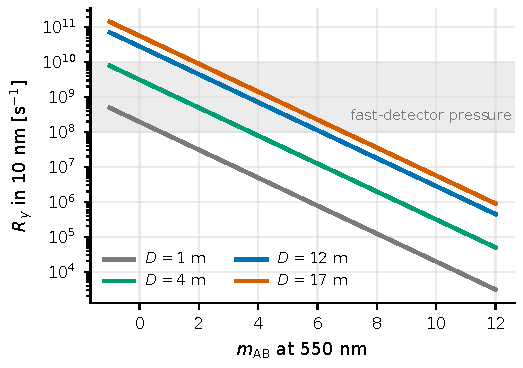
\includegraphics[width=0.86\linewidth]{figures/generated/chapter_18/ch18_photon_rate_magnitude.pdf}
\caption{AB 星等到窄带光子率的换算。曲线采用 550 nm、10 nm 通带、总效率 \(\eta=0.25\)。口径只线性改变收集面积，星等每增 5 等会让光子率降 100 倍；灰色区域标出 \(10^8\,{\rm s^{-1}}\) 以上、开始对高速探测和数据吞吐形成压力的区间。}
\label{fig:e15-photon-rate}
\end{figure}

\paragraph{相干稀释：为什么原始光子率不等于可用信号}

强度干涉真正要测的，是二阶相关在零延迟处的那个小小凸起，它的高度由光学\textbf{相干时间}\(\tau_c\)（coherence time，第 \ref{chap:e02} 章）和电子响应时间共同决定。相干时间是"光波还记得自己相位的时间"，由带宽定：\(\tau_c\simeq1/\Delta\nu\simeq\lambda^2/(c\,\Delta\lambda)\)。取 VERITAS 常用的 416 nm、13 nm 通带：
\[
  \tau_c\simeq\frac{\lambda^2}{c\,\Delta\lambda}
  =\frac{(416\times10^{-7})^2}{3\times10^{10}\times13\times10^{-7}}
  \approx 4.4\times10^{-14}\,{\rm s} .
\]
这是几十飞秒——比任何电子学快得多。而探测器加电子链的等效时间宽度是 \(\Delta t\sim4\,{\rm ns}\)。真正的相关峰只在 \(\tau_c\) 这么窄的时间里成立，却被摊平到 \(\Delta t\) 这么宽的时间 bin 里，于是峰高被稀释了约 \(\tau_c/\Delta t\)：
\[
  \frac{\tau_c}{\Delta t}\approx\frac{4.4\times10^{-14}}{4\times10^{-9}}
  \approx1.1\times10^{-5}.
\]
所以未解析热光在零基线上的归一化相关峰，自然落到几个 \(10^{-6}\) 的量级——这正是 VERITAS 论文里测到的 \(N_0\sim10^{-6}\) 那一档 \citep{2020NatAs...4.1164A,2024ApJ...966...28A}。峰这么矮，意味着它必须靠长时间平均和严格定标才能从噪声里"浮"出来。图 \ref{fig:e15-coherence} 把这层稀释画了出来。

\begin{figure}[tbp]
\centering
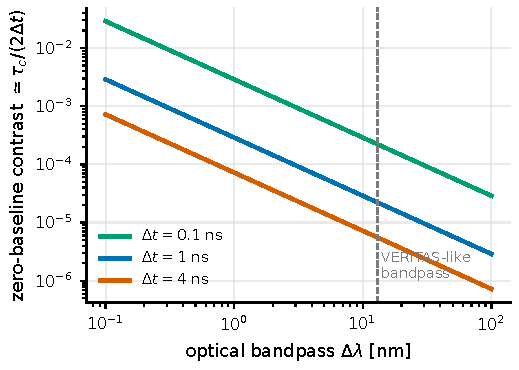
\includegraphics[width=0.86\linewidth]{figures/generated/chapter_18/ch18_coherence_dilution.pdf}
\caption{通带越宽，光学相干时间越短；电子时间分辨率越慢，零延迟相关峰越被稀释。416 nm、13 nm、4 ns 的组合给出几个 \(10^{-6}\) 的对比度，因此相关峰只能靠长积分和严格定标从噪声中显形。}
\label{fig:e15-coherence}
\end{figure}

这里藏着一个反直觉但极重要的事实：\textbf{把光学通带调宽，并不会按比例改善信噪比}。宽带确实让光子多了（\(R_\gamma\propto\Delta\lambda\)），但同时把相干时间缩短、把每个时间 bin 里的相关对比度压低（\(\propto\tau_c\propto1/\Delta\lambda\)）。两者在信噪比里几乎恰好抵消——下一节会看到这一点。真实仪器仍要挑滤光片，但那是为了控制 PMT 电流、天空背景、斜入射效应或选谱线，而不是简单地"越宽越好" \citep{2020MNRAS.491.1540A,2024MNRAS.529.4387A}。

\section{信噪比与积分时间怎么估}
\label{sec:e15-snr}

有了光子率，就能问最关心的问题：曝多久，信号才够强？第 \ref{chap:e11} 章推出的强度干涉信噪比标度是这一切的核心：

\begin{equation}
  {\rm SNR}
  = A\,\alpha\,n\,|V(\bm B)|^2\,
    \sqrt{\frac{\Delta f\,T}{2}} .
  \label{eq:e15-snr}
\end{equation}
\begin{formulaexplain}
\(A\)：收集面积（\({\rm cm^2}\)）。\(\alpha\)：量子效率（无量纲）。\(n\)：入射谱光子密度 \({\rm photons\,s^{-1}\,cm^{-2}\,Hz^{-1}}\)。\(|V|^2\)：平方可见度。\(\Delta f\)：电子带宽（Hz）。\(T\)：积分时间（s）。信号随 \(\sqrt{T}\) 攒起来。
\end{formulaexplain}

先把每个符号钉牢。\(A\) 是每台望远镜的有效面积（\({\rm cm^2}\)）；\(\alpha\) 是量子效率（无量纲）；\(n\) 是\textbf{入射谱光子密度}——单位面积、单位时间、单位光学带宽里的光子数，量纲 \({\rm photons\,s^{-1}\,cm^{-2}\,Hz^{-1}}\)，它由源的表面亮度（也就是亮温）决定，\emph{与你选多宽的光学通带无关}。\(|V(\bm B)|^2\) 是基线 \(\bm B\) 上的平方可见度（无量纲，介于 0 与 1），是我们真正想测的目标信号。\(\Delta f\) 是电子带宽（Hz），由光脉冲、PMT/SPAD 响应、线缆、放大器、数字化器和软件相关共同决定的等效带宽。\(T\) 是积分时间（s）。

这条式子有几处值得咀嚼。第一，把 \(A\,\alpha\,n\) 合起来看：它的量纲是 \({\rm s^{-1}\,Hz^{-1}}\)，而 \({\rm Hz^{-1}=s}\)，所以整体\emph{无量纲}——它就是每个模式里的平均光子占据数 \(\delta=A\alpha n\)，即\textbf{光子简并度}（photon degeneracy）。可见光热星的 \(\delta\) 只有 \(10^{-4}\)--\(10^{-2}\)，这正是强度干涉信号如此微弱的根源。第二，因为 \(n\) 是\emph{谱}密度，加宽光学通带并不改 \(n\)——这就从公式上证实了上一节那句"宽带不白赚信噪比"。第三，也是最实用的一条：\({\rm SNR}\propto\sqrt{T}\)。信号不是线性攒的，是\emph{开方}攒的——要把信噪比翻倍，得曝四倍长的时间。这条 \(\sqrt{T}\) 定律下一节会成为误差预算的主角。

代一个真实场景。LeBohec 与 Holder 取 \(A=100\,{\rm m^2}\)、\(\alpha=0.3\)、\(\Delta f=1\,{\rm GHz}\)、\(T=5\,{\rm h}=1.8\times10^4\,{\rm s}\)、\(|V|^2=0.5\)，算得一颗 \(m_V\simeq6.7\) 的星恰好落在 \(5\sigma\) 一档；同样条件下 \(m_V=5\) 的星（亮 1.7 等、\(n\) 大约 5 倍）信噪比冲到二十以上，而 \(m_V=9\) 的星只剩不到 \(1\sigma\)，等于测不出 \citep{2006ApJ...649..399L,2008AIPC..984..205L}。把这套依赖画成星等\,--\,积分时间的热图，就是图 \ref{fig:e15-snr}。要反过来求积分时间也很直接：把式 \eqref{eq:e15-snr} 解出 \(T\)，
\[
  T = \frac{2\,{\rm SNR}^2}{(A\alpha n)^2\,|V|^4\,\Delta f},
\]
即所需时间随目标信噪比\emph{平方}增长、随简并度平方和可见度四次方\emph{反比}下降——这解释了为什么暗一点、或已被高度解析（\(|V|^2\) 很小）的目标，会让积分时间迅速失控。

\begin{figure}[tbp]
\centering
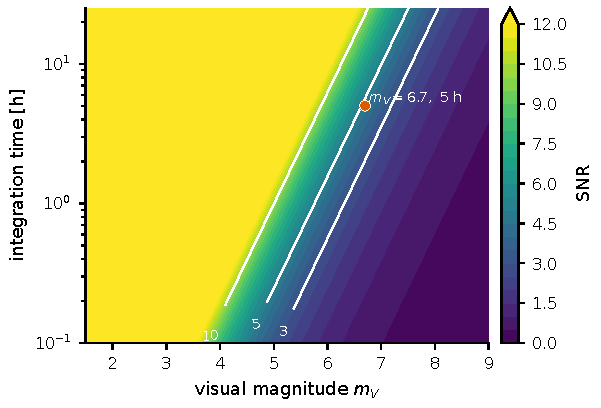
\includegraphics[width=0.90\linewidth]{figures/generated/chapter_18/ch18_snr_heatmap.pdf}
\caption{强度干涉信噪比对星等和积分时间的依赖。图中取 \(A=100\,{\rm m^2}\)、\(\alpha=0.3\)、\(\Delta f=1\,{\rm GHz}\)、\(|V|^2=0.5\)；橙点对应 LeBohec--Holder 估算里 \(m_V\simeq6.7\)、5 h 约 \(5\sigma\) 的位置。}
\label{fig:e15-snr}
\end{figure}

用式 \eqref{eq:e15-snr} 做第一轮估算时要记住它是"理想版"。真实数据里，\(T\) 是过了质量切片后的有效曝光时间（live time），不是挂钟时间；\(\Delta f\) 是整条电子链的等效带宽；\(|V|^2\) 还会随目标高度和时角缓慢变化。举一组真实工程数字：VERITAS 用四台 12 m 望远镜同时给出六条基线，配 416 nm、约 13 nm 滤光片和 4 ns 采样，每小时吐出约 3.5 TB 原始数据；MAGIC 用两台 17 m 望远镜和中央 PMT，早期演示报告的灵敏度比 Narrabri 高约一个量级。而 Vega 光子计数实验走的是另一条路——用单光子雪崩二极管（SPAD）加软件相关，在零基线测到 \(\langle g^{(2)}\rangle=1.0034\pm0.0008\)，在约 2 km 投影基线上则\emph{不}出现相关，正符合 Vega 约 3.3 mas 的角直径在那条基线上已被完全解析的预期 \citep{2020NatAs...4.1164A,2020MNRAS.491.1540A,2021MNRAS.506.1585Z}。

多台望远镜同时买到两样东西：更多数据、更多几何。\(N\) 台望远镜给出 \(N(N-1)/2\) 条同时基线——4 台只有 6 条，60 台就有 1770 条。关键是，不同基线是在 \(u,v\) 平面的\emph{不同点}上采样源结构，绝非重复测量同一个数（第 \ref{chap:e11} 章）。测均匀圆盘直径，几条合适基线就够；但要测快速自转星的扁率、双星、盘风或非轴对称的谱线发射区，就非要位置角覆盖不可。覆盖 0.1--3 mas 的热星结构时，30--2000 m 这一整段基线范围，比单纯堆一条最长基线更有用。图 \ref{fig:e15-uv} 对比了小阵列与大阵列的 \(u,v\) 覆盖。

\begin{figure}[tbp]
\centering
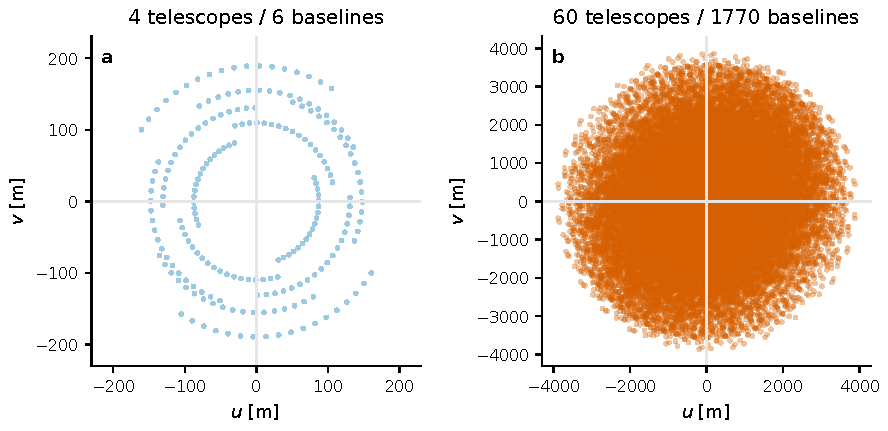
\includegraphics[width=0.94\linewidth]{figures/generated/chapter_18/ch18_uv_coverage.pdf}
\caption{阵列规模怎样改变 \(u,v\) 采样。左：四台望远镜的六条基线，随时角旋转后仍较稀疏；右：多望远镜阵列，短、中、长基线同时存在。密集覆盖不自动等于高信噪比，但它决定非轴对称目标能否被稳定拟合或重建。}
\label{fig:e15-uv}
\end{figure}

\section{基线、带宽与波段的选择由可见度斜率决定}
\label{sec:e15-baseline}

已经有了信噪比，为什么还不能马上定基线？因为\textbf{信号强}和\textbf{信息多}是两回事。一条基线可能相关峰很高（信噪比很好），却对我们想测的角直径几乎不敏感——这时它测得再准也没用。要判断"哪条基线才携带直径信息"，得看可见度曲线的\emph{斜率}。

先把角尺度和基线的粗关系摆出来。要分辨角尺度 \(\theta\)，需要的基线约为

\begin{equation}
  B\sim\frac{\lambda}{\theta}
  = 86\,{\rm m}\left(\frac{\lambda}{416\,{\rm nm}}\right)
                \left(\frac{1\,{\rm mas}}{\theta}\right).
  \label{eq:e15-baseline}
\end{equation}
\begin{formulaexplain}
\(B\)：所需基线（m）。\(\lambda\)：观测波长。\(\theta\)：目标角尺度（这里以 mas 为单位）。这是量级式：要分辨越小的角，需要越长的基线；波长越短，同样基线分辨越细。
\end{formulaexplain}

代几个数就有画面了：\(\theta=2\,{\rm mas}\) 的热星在 416 nm 只要约 43 m 就开始被解析；\(\theta=0.5\,{\rm mas}\) 要约 170 m；\(\theta=0.1\,{\rm mas}\) 得进到约 860 m。Narrabri 的最大基线约 188 m，所以它最擅长又亮又热、角直径在零点几到几 mas 的星；CTA 级的公里阵列能把空间频率推到几十微角秒，但目标还得有足够光子率才玩得起 \citep{1974MNRAS.167..121H,2006ApJ...649..399L}。

现在看斜率。均匀圆盘（第 \ref{chap:e11} 章）的平方可见度随基线先是接近 1 的平台，然后下降，在第一零点处触底。观测设计的要害在于：如果你所有基线都落在 \(|V|^2\simeq1\) 的平台上，不同 \(\theta\) 的曲线几乎重合，你根本分不出星的大小；如果你只测第一零点\emph{之后}的极低可见度，相关峰又低到贴着噪声。\textbf{直径信息集中在曲线下降最陡、也就是斜率 \(|\partial|V|^2/\partial\theta|\) 最大的那一段基线}——通常在第一 lobe 的下降区和第一零点附近。所以一份严肃的可行性计算，不但要画目标模型的 \(|V|^2(B)\)，还要画它对参数的导数 \(\partial|V|^2/\partial\theta\)，看峰值落在哪条基线（图 \ref{fig:e15-vis}）。

\begin{figure}[tbp]
\centering
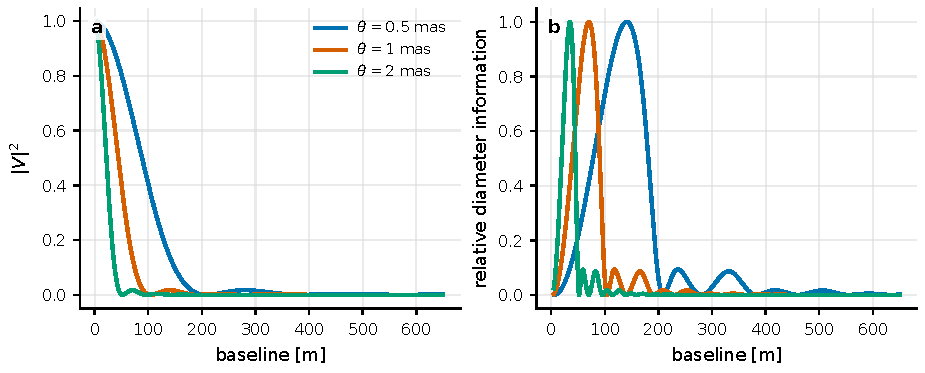
\includegraphics[width=0.94\linewidth]{figures/generated/chapter_18/ch18_visibility_fisher.pdf}
\caption{均匀圆盘的平方可见度曲线与直径灵敏度。416 nm 下，2 mas、1 mas、0.5 mas 目标的下降区分别落在几十米、百米、几百米基线；右图显示直径信息主要来自曲线斜率大的基线，短基线平台 \(|V|^2\simeq1\) 对直径几乎不敏感。}
\label{fig:e15-vis}
\end{figure}

把这层直觉写成公式，就是第 \ref{chap:e12} 章的 Fisher 信息。对单个参数 \(\theta\)、一组独立基线测量 \(\mu_i=|V_i|^2\)，Fisher 信息与可达方差为

\begin{equation}
  I(\theta)=\sum_i
  \frac{1}{\sigma_i^2}
  \left(\frac{\partial\mu_i}{\partial\theta}\right)^{\!2},
  \qquad
  \sigma_\theta\ge\frac{1}{\sqrt{I(\theta)}} .
  \label{eq:e15-fisher}
\end{equation}
\begin{formulaexplain}
\(\mu_i\)：第 \(i\) 条基线上的可测量（如 \(|V_i|^2\)）。\(\partial\mu_i/\partial\theta\)：它对目标参数的灵敏度（斜率）。\(\sigma_i\)：该测量的误差。右式是 Cramér--Rao 下界。斜率大、误差小的基线，贡献最大。
\end{formulaexplain}

这条式子把前面几句话变成了可算的判据。每条基线的贡献是\emph{斜率平方除以误差平方}：斜率 \(\partial\mu_i/\partial\theta\) 大、误差 \(\sigma_i\) 小，才贡献得多。于是两种"看着不错却没用"的基线立刻现形——误差再小、但斜率近零（平台上）的基线，贡献几乎为零；斜率再大、但 \(|V|^2\) 太低导致相关峰淹在噪声里、\(\sigma_i\) 巨大的基线，也撑不起结果。注意 \(\sigma_i\) 里既要放统计噪声（来自式 \eqref{eq:e15-snr}），也要放下一节的系统项。VERITAS 对快速自转星 \(\gamma\) Cas 的观测就是活例子：不同投影基线采样不同方向的 \(|V|^2\)，才约束出扁率和长轴方向，单一个等效圆盘直径根本描述不了这种非轴对称目标 \citep{2025ApJ...995..191A,2024ApJ...966...28A}。

波段选择跟着一起决定。同一条物理基线，在 416 nm 采到的空间频率比 800 nm 高约 1.9 倍——蓝端分辨率更高，但大气透过、镜面反射、探测器量子效率和滤光片斜入射都更难对付。谱线观测则要换一套账：算的是线通量而非宽带星等。对热星和 Be 星，H\(\alpha\)、氦线或金属线可能来自比连续谱更大的发射区；用窄带把几何结构和速度通道分开是值得的，但每个通道的事件率、滤光片泄漏和背景都得重新算过 \citep{2012NewAR..56..143D,2021MNRAS.506.1585Z}。

\section{误差预算：统计地板与系统地板}
\label{sec:e15-error-budget}

现在到了整章最实用、也最容易被外行忽略的一节。新手写观测申请，往往只报一个信噪比就完事。但信噪比只管\emph{统计}噪声，它会随积分时间一路下降；真正决定"你到底能测多准"的，常常是一层\textbf{不随时间下降的系统地板}。把两者分开，就是误差预算。

对一个待拟合参数 \(\theta\)，把各路误差按方差相加：

\begin{equation}
  \sigma_\theta^2
  = \sigma_{\rm stat}^2
  + \sigma_{\rm bg}^2
  + \sigma_{\rm time}^2
  + \sigma_{\rm cal}^2
  + \sigma_{\rm model}^2 .
  \label{eq:e15-error-budget}
\end{equation}
\begin{formulaexplain}
\(\sigma_\theta\)：目标参数的总误差。右边依次是统计、背景、时间、定标、模型误差。它们独立时按方差相加。这条式子提醒你：报一个信噪比不够，还得说清误差平台从哪来。
\end{formulaexplain}

逐项说清它们各是什么、量纲都折算到 \(\theta\) 的单位上。\(\sigma_{\rm stat}\) 来自有限的符合计数或相关峰拟合，是式 \eqref{eq:e15-snr} 那个信噪比的直接后果。\(\sigma_{\rm bg}\) 来自离源背景（off-source）插值和暗电流的不确定。\(\sigma_{\rm time}\) 来自时钟、几何延迟、采样和峰形。\(\sigma_{\rm cal}\) 来自校准星、系统总透过率、滤光片和偏振。\(\sigma_{\rm model}\) 来自源模型本身——把快速自转星硬当成圆盘、把谱线盘硬当成高斯、或忽略一颗伴星，都会引入这项。

关键的物理在于它们\emph{随时间的行为不同}。统计项遵守散粒噪声的 \(\sqrt N\) 定律（第 \ref{chap:e03} 章）：计数 \(N\propto T\)，所以

\begin{equation}
  \sigma_{\rm stat}(T)=\frac{c_0}{\sqrt{T}} ,
  \qquad
  \sigma_{\rm sys}^2=\sigma_{\rm bg}^2+\sigma_{\rm time}^2
        +\sigma_{\rm cal}^2+\sigma_{\rm model}^2 ,
  \label{eq:e15-floor}
\end{equation}
\begin{formulaexplain}
\(c_0\)：由光子率、可见度斜率等决定的常数。\(\sigma_{\rm stat}\propto T^{-1/2}\) 随曝光下降；\(\sigma_{\rm sys}\) 把不随时间下降的系统项合在一起。总误差是两者的方差和。
\end{formulaexplain}

这里 \(c_0\) 是把光子率、可见度斜率、定标链一并吸收进去的常数（单位与 \(\theta\) 一致）。图像很清楚：\(\sigma_{\rm stat}\) 像一条不断下滑的斜坡，随你曝得越久越低；而 \(\sigma_{\rm sys}\) 是一块\emph{水平的地板}。总误差是二者的方差和，一开始被统计斜坡主导、随 \(T\) 下降，直到撞上系统地板就\emph{不动了}。撞上的时刻，就是统计项等于系统项的那一刻：
\[
  \sigma_{\rm stat}(T_\star)=\sigma_{\rm sys}
  \;\Longrightarrow\;
  T_\star=\left(\frac{c_0}{\sigma_{\rm sys}}\right)^{2}.
\]
\textbf{曝到 \(T_\star\) 以后再加时间，几乎白费}——总误差已经贴着系统地板，你把 \(T\) 再翻四倍，统计项才减半，而它早已远小于地板，对总误差毫无影响。这就是可行性计算里最该讲清、也最该写进申请的一句话：不是"曝得越久越好"，而是"曝到统计项降到系统地板附近就该停，剩下的精度要靠压低系统项去争"。图 \ref{fig:e15-budget} 把这条斜坡撞地板的行为画了出来。

\begin{figure}[tbp]
\centering
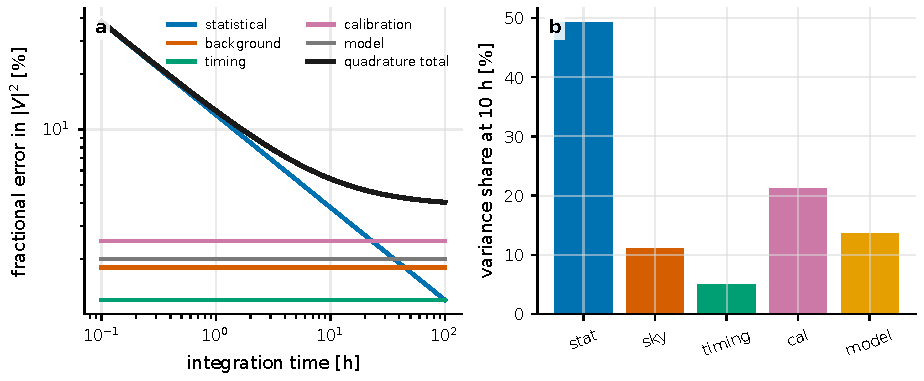
\includegraphics[width=0.94\linewidth]{figures/generated/chapter_18/ch18_error_budget.pdf}
\caption{误差预算里的统计项与系统项。左：统计误差随积分时间下降，但背景、时间、定标、模型项合成一块平台；右：10 h 时各项对总方差的贡献。观测申请应把每一项都连到一份可观测的定标数据，并在总信噪比之外给出误差平台。}
\label{fig:e15-budget}
\end{figure}

系统项里最常见、也最好量化的一项是\textbf{背景稀释}。若源外还有一份与信号\emph{不相关}的背景光（天光、月光、暗计数），它不会造出假相关，却会把真相关峰按比例压低。设某端背景与星光之比为 \(\beta\)，两端对称时观测到的对比度按 \((1+\beta)^{-2}\) 缩水（第 \ref{chap:e08} 章）。代数字：\(\beta=0.03\)（背景只有星光的 3\%）时 \((1.03)^{-2}=0.94\)，只掉 6\%，几乎无害；但 \(\beta=0.5\) 时 \((1.5)^{-2}=0.44\)，峰只剩原来的四成多。VERITAS 对 \(\beta\) UMa 的分析，用目标附近 0.5\(^\circ\) 的离源观测（off runs）估非星光电流，典型离源强度只有在源的约 3\%，所以对半径拟合影响很小；可一旦有明月、云、雾、城市灯光或探测器后脉冲（afterpulsing），这个近似就变差，得单独做质量切片 \citep{2024ApJ...966...28A,2025ApJ...995..191A}。图 \ref{fig:e15-bg} 给出稀释因子及其反向修正。

\begin{figure}[tbp]
\centering
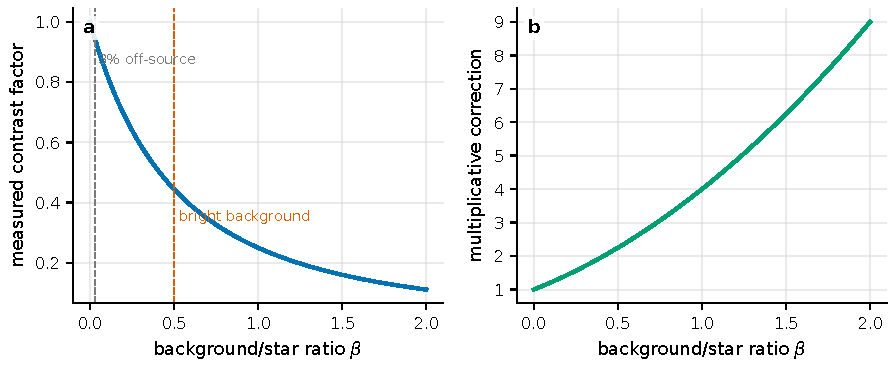
\includegraphics[width=0.94\linewidth]{figures/generated/chapter_18/ch18_background_dilution.pdf}
\caption{不相关背景对相关峰的稀释。两端背景/星光比相同时，观测对比度按 \((1+\beta)^{-2}\) 下降：\(\beta=0.03\) 只造成几个百分点修正，\(\beta=0.5\) 已把峰压到约 44\%。右图是反向修正因子，修正越大，对背景估计误差越敏感。}
\label{fig:e15-bg}
\end{figure}

时间定标是强度干涉和光子计数共同的硬边界。相关峰宽通常几纳秒；若两台望远镜的相对延迟模型错了 1 ns，峰就会被摊宽、甚至移出拟合窗口。Vega 光子计数实验里，零基线子孔径的相对时间精度约 100 ps，两台望远镜之间还要处理光行时、仪器延迟、GPS 或铷钟漂移和光纤色散，最后用约 400 ps 的时间 bin 做相关；他们明确指出多望远镜方案要做到约纳秒级同步，才能把观测时间维持在小时量级。VERITAS 用 White Rabbit 的 10 MHz 时钟分发加 4 ns 采样，仍要在每个 run 里跟踪光程延迟随时角的漂移，并处理 run 到 run 的峰位变化 \citep{2021MNRAS.506.1585Z,2024ApJ...966...28A}。

校准星（calibrator）要跟科学目标一样认真选。理想的校准星应有已知角直径、稳定光度、贴近目标的天区位置、相近颜色和足够高的光子率。若目标是 0.5 mas 的热星，而校准星直径本身有 5\% 的不确定，那么最终直径误差很容易被这一项 \(\sigma_{\rm cal}\) 主导——曝再久也没用。现代强度干涉观测常先拿已知角直径的热星当参考，核对零基线归一化、滤光片响应和 \(|V|^2(B)\) 形状，再去测未知目标。MAGIC 2024 年的性能论文就用多颗参考星验证系统，再给出新恒星角直径；VERITAS 从 \(\beta\) UMa 的圆盘直径一路走到 \(\gamma\) Cas 的扁率和位置角，用的也是同一套定标框架 \citep{2024MNRAS.529.4387A,2024ApJ...966...28A,2025ApJ...995..191A}。

\section{一次从头到尾的可行性计算}
\label{sec:e15-worked}

现在把整章串成一次真实的算。设科学目标是：\textbf{用 VERITAS 型阵列测量一颗热亮星的角直径，把相对误差压到百分之几}。阵列参数全部取自真实的 VERITAS 强度干涉系统；目标取一颗落在灵敏度边缘的热星，好让这道题既不是"轻松能测"也不是"根本没戏"。

\textbf{第 0 步：写下目标参数与成功标准。}要测的物理量是角直径 \(\theta\)，目标精度 \(\sigma_\theta/\theta\lesssim3\%\)。成功标准量化为：至少三条基线在第一 lobe 下降区达到 \({\rm SNR}>5\)；校准星重复观测的归一化漂移小于 3\%；离源背景修正小于总信号的 10\%。

\textbf{第 1 步：选目标，定光子率。}我们特意挑一颗比 \(\beta\) UMa（\(m_V\approx2.4\)）、\(\gamma\) Cas（\(m_V\approx2.2\)）这些 VERITAS 真实亮目标更暗、正落在灵敏度边缘的 \(m_V\approx5\) 假想早型星，有效温度约 \(10^4\,{\rm K}\)，好让这道题不至于太轻松。（提醒一句：本节用到的 \(m_V\approx5\)、\(T_{\rm eff}\approx10^4\,{\rm K}\)、\(\theta\approx0.7\,{\rm mas}\) 是为演示各步骤而\emph{各自独立给定}的示意数，不必对应同一颗真实恒星——若认真代进 Stefan--Boltzmann 关系 \(f_{\rm bol}=\sigma T^4(\theta/2)^2\)，会发现这三个数并不严格自洽，读者不必纠结于此。）用第 \ref{sec:e15-photon-budget} 节的链条，一台 12 m 望远镜在 550 nm、10 nm 通带、\(\eta=0.25\) 下给出 \(R_\gamma\simeq2.8\times10^8\,{\rm s^{-1}}\)。换到 VERITAS 实际的 416 nm、13 nm 滤光片，光子率同量级。结论：光子够多，这颗星不会因为太暗而出局。

\textbf{第 2 步：估角尺度，定基线。}\(10^4\,{\rm K}\) 的早型亮星角直径通常在 0.5--1 mas。由式 \eqref{eq:e15-baseline}，在 416 nm 下 \(\theta\approx0.7\,{\rm mas}\) 的星，第一 lobe 下降区落在约 \(86/0.7\approx120\,{\rm m}\) 一带。VERITAS 四台 12 m 望远镜的六条基线覆盖几十米到约 170 m，正好把下降区和第一零点附近都罩住——这意味着我们有几条基线落在\emph{斜率大}的位置上，符合第 \ref{sec:e15-baseline} 节的直径信息判据。

\textbf{第 3 步：估相关峰高与统计信噪比。}由第 \ref{sec:e15-photon-budget} 节，416 nm、13 nm、4 ns 给出 \(\tau_c\simeq4.4\times10^{-14}\,{\rm s}\)、稀释后的零基线峰约几个 \(10^{-6}\)。把阵列参数代入式 \eqref{eq:e15-snr}：LeBohec--Holder 的等效计算表明，\(A=100\,{\rm m^2}\)、\(\alpha=0.3\)、\(\Delta f=1\,{\rm GHz}\)、\(|V|^2=0.5\) 时，\(m_V\simeq6.7\) 的星 5 h 达到 \(5\sigma\)；我们这颗 \(m_V\approx5\) 的星亮约 5 倍，同样 5 h 的单基线信噪比可冲到二十以上。取保守的单基线 \({\rm SNR}\approx5\)--\(10\) 已足够。

\textbf{第 4 步：把信噪比翻译成角直径误差。}相关峰的相对误差是 \(\sigma_{|V|^2}/|V|^2\approx1/{\rm SNR}\)。要把它换成角直径的误差，用一次\textbf{误差传播}（error propagation）：可测量 \(|V|^2\) 是 \(\theta\) 的函数，\(\theta\) 的小误差经导数搬运成 \(|V|^2\) 的误差，
\[
  \sigma_{|V|^2}=\left|\frac{\partial|V|^2}{\partial\theta}\right|\,\sigma_\theta .
\]
把这条式子两边同时除以 \(|V|^2\) 与 \(\theta\)，右边正好凑成对数导数 \(\partial\ln|V|^2/\partial\ln\theta=(\theta/|V|^2)\,\partial|V|^2/\partial\theta\)，于是
\[
  \frac{\sigma_\theta}{\theta}
  =\frac{\sigma_{|V|^2}/|V|^2}{\left|\partial\ln|V|^2/\partial\ln\theta\right|} .
\]
在下降区，可见度对直径的\emph{对数斜率}\(|\partial\ln|V|^2/\partial\ln\theta|\) 是 1--2 量级；代入 \(\sigma_{|V|^2}/|V|^2\approx1/{\rm SNR}\)，得
\[
  \frac{\sigma_\theta}{\theta}
  \approx\frac{1}{{\rm SNR}}\,
  \frac{1}{\left|\partial\ln|V|^2/\partial\ln\theta\right|}
  \approx\frac{1}{5}\times\frac{1}{1.5}
  \approx13\%
\]
——\emph{单条}斜率大的基线，5 h 大约给到十几个百分点。再用式 \eqref{eq:e15-fisher} 把多条基线的信息相加：\(N_b\) 条同等有用的基线让统计误差按 \(1/\sqrt{N_b}\) 缩小，六条基线里若有三条落在下降区，\(\sigma_\theta/\theta\) 就压到约 \(13\%/\sqrt3\approx7\%\)；再叠几个夜晚或用更多台望远镜的更多基线，进到 3\% 是现实的。这一步把"信噪比"真正落成了"角直径能测到百分之几"。

\textbf{第 5 步：核对误差预算，判断该不该继续曝。}用式 \eqref{eq:e15-error-budget} 和 \eqref{eq:e15-floor} 检查系统地板。背景：离源 \(\beta\approx0.03\)，稀释修正约 6\%，且可由离源观测标定，\(\sigma_{\rm bg}\) 小。时间：White Rabbit 加 4 ns 采样，相对延迟控制在纳秒级，\(\sigma_{\rm time}\) 可控。定标：若校准星直径已知到 3\%，则 \(\sigma_{\rm cal}\) 约 3\%——这恰好和我们的目标精度同量级，成为\textbf{最可能的系统地板}。据式 \eqref{eq:e15-floor}，当统计项 \(\sigma_{\rm stat}\) 曝到降至约 3\% 时（对应 \(T_\star\)），总误差就贴着这块由校准星决定的地板，\emph{再加曝光已无意义}。结论直白：这次观测能否达到 3\%，最后不取决于再曝几小时，而取决于\emph{有没有一颗直径足够确定的校准星}。

\textbf{第 6 步：写成申请里的可行性结论。}一句话收束：目标 \(m_V\approx5\)、\(\theta\approx0.7\,{\rm mas}\) 的热星，用 VERITAS 六条基线、416 nm/13 nm、4 ns 采样，数个夜晚的有效曝光可在下降区多条基线上达到 \({\rm SNR}>5\)，把角直径统计误差压到约 3\%；系统地板由校准星直径不确定（约 3\%）主导，因此升级方向不是更长曝光，而是更好的校准星与更严的滤光片/背景控制。若最长基线未检出相关，仍能给出角直径\emph{上限}或排除过大的发射区——空手而归也是有价值的结果。

这条估算链并不专属强度干涉。振幅干涉、量子网络望远镜、CMB 偏振、快速射电暴（FRB）的光子统计，乃至实验室教学台架，都套同一副骨架：事件率 \(\to\) 模式数 \(\to\) 响应函数 \(\to\) 定标项 \(\to\) 模型导数 \(\to\) 误差预算；差别只在可测量 \(\mu_i\) 的具体形式。科学案例排序也该沿用这条思路，把"科学价值"和"可观测性"分成两栏各自打分，别把\emph{漂亮的}目标和\emph{做得成的}目标混为一谈 \citep{2010SPIE.7734E..0AD,2012MNRAS.419..172N,2013APh....43..331D,2022SPIE12183E..0DK}。表 \ref{tab:e15-checklist} 把这份账本里每个量的常见范围和用法列成一张清单。

\begin{longtable}{p{0.16\linewidth}p{0.30\linewidth}p{0.44\linewidth}}
\caption{可行性账本速查表：每个量的常见范围与在计划中的用法。}
\label{tab:e15-checklist}\\
\toprule
量 & 常见范围 & 在计划中的用法 \\
\midrule
\endfirsthead
\toprule
量 & 常见范围 & 在计划中的用法 \\
\midrule
\endhead
\(m_V,\,m_B\) & \(-1\) 到 \(9\) 等，是当前强度干涉的主战场 & 经式 \eqref{eq:e15-ab-flux} 与 \eqref{eq:e15-photon-rate} 转成 \(R_\gamma\)，先判断目标是否过暗。 \\
\(A_{\rm eff}\) & 每台 \(1\)--\(250\,{\rm m^2}\) & 进入光子率与信噪比；镜面老化、遮挡、光纤耦合都要折进效率。 \\
\(\Delta\lambda\) & \(0.1\)--\(30\,{\rm nm}\) & 决定相干时间、PMT 电流、天空背景与谱线选择。 \\
\(\Delta t\) & \(0.1\)--\(5\,{\rm ns}\) & 决定相关峰被稀释的程度和可用电子带宽。 \\
\(B_p\) & \(10\)--\(2000\,{\rm m}\) & 决定角尺度和 \(u,v\) 覆盖；短、长基线约束不同结构。 \\
\(\beta\) & \(0.01\)--\(1\) & 背景/星光比，决定对比度稀释与背景系统误差。 \\
\(\sigma_{\rm cal}\) & 可见度或直径的 \(1\%\)--\(10\%\) & 常成为长曝光后的误差地板。 \\
\bottomrule
\end{longtable}

\section{本章要点}
\label{sec:e15-summary}

\begin{itemize}
  \item \textbf{观测是一张账本。}式 \eqref{eq:e15-likelihood} 把物理参数经"仪器可测量 + 定标 + 背景"连到数据；设计观测就是逐段把这条链算成真实数字，而不是只写"要看哪颗星"。事件表是原汤，图像是熬干的一勺——记录时被平均掉的信息补不回来。
  \item \textbf{光子预算分四步。}星等 \(\to\) 谱流量密度（式 \eqref{eq:e15-ab-flux}）\(\to\) 单位面积光子通量 \(\to\) 乘面积与效率得有效光子率（式 \eqref{eq:e15-photon-rate}）。一台 12 m 望远镜对 \(m_{\rm AB}=5\) 的星给出 \(R_\gamma\simeq2.8\times10^8\,{\rm s^{-1}}\)；但相干稀释 \(\tau_c/\Delta t\sim10^{-5}\) 把零基线峰压到几个 \(10^{-6}\)。
  \item \textbf{信噪比按 \(\sqrt T\) 攒。}式 \eqref{eq:e15-snr} 里 \({\rm SNR}\propto A\alpha n|V|^2\sqrt{\Delta f\,T}\)；\(A\alpha n\) 就是光子简并度 \(\delta\sim10^{-4}\)--\(10^{-2}\)。因为 \(n\) 是谱密度，加宽光学通带几乎不白赚信噪比。要精度翻倍得曝四倍时间。
  \item \textbf{基线由可见度斜率选。}直径信息集中在 \(|\partial|V|^2/\partial\theta|\) 最大的下降区（式 \eqref{eq:e15-fisher}）；平台上斜率近零的基线，误差再小也没贡献，可见度太低的基线，斜率再大也淹在噪声里。
  \item \textbf{误差预算 = 统计地板 + 系统地板。}式 \eqref{eq:e15-error-budget} 与 \eqref{eq:e15-floor}：\(\sigma_{\rm stat}\propto T^{-1/2}\) 一路下滑，系统项（背景、时间、定标、模型）是一块水平地板。曝到 \(T_\star=(c_0/\sigma_{\rm sys})^2\)、统计项撞上地板后，\emph{再加曝光已无意义}——剩下的精度要靠压低系统项去争。
  \item \textbf{可行性计算有固定套路。}目标参数 \(\to\) 光子率 \(\to\) 基线 \(\to\) 信噪比 \(\to\) 角直径误差 \(\to\) 误差预算判停。这套骨架同样适用于振幅干涉、量子网络望远镜、CMB 偏振和 FRB 光子统计，差别只在可测量的形式。
\end{itemize}

\medskip
\noindent\textbf{想一想。}
(1) 若把光学通带从 10 nm 加宽到 30 nm，光子率涨 3 倍，可强度干涉的信噪比几乎不动——用式 \eqref{eq:e15-snr} 里 \(n\) 是谱密度这一点解释为什么。
(2) 你已经曝了 5 h，统计误差 4\%，但校准星直径只知到 3\%。再曝到 20 h 值不值？用式 \eqref{eq:e15-floor} 算一算总误差会从多少降到多少。
(3) 一颗星的角直径估计是 0.3 mas，你手上最长基线只有 100 m（416 nm）。你落在可见度曲线的哪一段？这条基线对直径敏感吗？该往长还是往短要基线？
